% IMMI-formatted version of the projection-law paper.
% Format-free initial submission per Springer practice; structured abstract,
% numbered citations, single column, declarations block per IMMI conventions.
% The PRX-formatted master is ../projection-law.tex — keep content in sync.
\documentclass[11pt]{article}
\usepackage[utf8]{inputenc}
\usepackage[T1]{fontenc}
\usepackage{amsmath,amssymb,amsthm}
\usepackage{booktabs}
\usepackage{graphicx}
\usepackage[margin=2.5cm]{geometry}
\usepackage[numbers,sort&compress]{natbib}
\usepackage{hyperref}
\hypersetup{colorlinks=true, linkcolor=blue, citecolor=blue, urlcolor=cyan}
\graphicspath{{../figures/}}

\newtheorem{theorem}{Theorem}
\newcommand{\inn}[2]{\langle #1, #2 \rangle}

\title{\bfseries The Projection Law: Model-Ensemble Errors Point at Their Binding Constraint}
\author{Alex Welcing\\ \small Lupine Science, New York, NY\\ \small \texttt{alex@lupine.io}\\[2pt]
\small ORCID: 0009--0000--0000--0000 (to be completed)}
\date{}

\begin{document}
\maketitle

\begin{abstract}
\noindent\textbf{Purpose:} Multi-model agreement is routinely used as
confidence in materials simulation and beyond, yet models in a family share
construction and training lineage. This work formalizes and tests the
projection law: a model family acts as a projection operator, every
well-fitted member shares one residual --- a single direction in observable
space --- and that direction fingerprints whatever constraint binds the
family.
\textbf{Methods:} The theoretical core (normal-cone consensus theorem;
participation-ratio gauge $\mathrm{PR}(d,\rho)=(\rho+d)^2/((\rho+1)^2+(d-1))$
with explicit ribbon-collapse rate; ribbon/consensus decoupling) is
machine-checked in Lean~4 with zero unproven obligations. Two factorial
experiments were pre-registered with refutation conditions committed before
execution: a $4{\times}2$ architecture-by-functional crossing of MatPES-trained
foundation interatomic potentials evaluated on elastic constants of 15 cubic
metals, and an analysis of 12 DFT implementations on 384 equation-of-state
benchmarks from the ACWF verification effort. A two-tier replication kit
verifies every statistic from committed raw data (NumPy only, seconds) and
re-derives the raw data from public checkpoints (bit-exact).
\textbf{Results:} Foundation-model errors cluster by training functional, not
architecture ($S_{\mathrm{func}}{=}{+}0.317$ vs.\
$S_{\mathrm{arch}}{=}{-}0.093$, exact permutation $p{=}0.029$); r$^2$SCAN
training rotates noble-metal $C_{44}$ errors toward experiment as predicted.
DFT-implementation errors cluster by pseudopotential table, not simulation
code ($S_{\mathrm{table}}{=}{+}0.526$ vs.\ $S_{\mathrm{code}}{=}{+}0.265$,
$p{=}0.017$); four independent plane-wave codes sharing one table align at
$0.70$--$0.87$. Neither registered refutation condition was triggered.
Combined with the 559-potential classical baseline (within-family error
correlation $0.95$; error dimensionality invariant over forty years), error
anisotropy is conserved across paradigm replacements while its direction
rotates to the next constraint upstream. A single shared correction vector
removes ${\sim}96\%$ (median) of foundation-model elastic-constant error.
\textbf{Conclusion:} Agreement among models sharing a constraint measures the
constraint, not the truth. Error-vector geometry converts benchmarking from
scoring into diagnosis, supplies a zero-cost trust rule for ensemble
uncertainty, and enables family-level calibration without retraining.
\end{abstract}

\noindent\textbf{Keywords:} model ensembles; error geometry; uncertainty
quantification; interatomic potentials; foundation models; density functional
theory; verification and validation; benchmarking; formal methods

\section{Introduction}

Every field that builds models in families uses inter-model agreement as
evidence. The practice has long been questioned qualitatively: climate
ensembles share construction and history, so their consensus may reflect
common structure rather than truth \citep{pirtle2010,parker2011}, and error
correlations between members quantify that dependence
\citep{bishop2013,annan2011,knutti2013}. In machine learning, independently
trained networks agree far beyond what their accuracy predicts
\citep{mania2019,geirhos2020}, ensemble members cluster in prediction space
\citep{fort2019}, and disagreement tracks the shared bias of the training
procedure rather than correctness \citep{jiang2021}. In materials simulation
specifically --- the substrate of this work --- ensembles of interatomic
potentials have served as error estimators since Frederiksen et
al.~\citep{frederiksen2004}, universal machine-learned interatomic potentials
(MLIPs) are known to share a systematic softening inherited from their
training data \citep{deng2025softening,yu2024}, and the reproducibility of
density-functional-theory (DFT) implementations is monitored by scalar
metrics \citep{lejaeghere2016,bosoni2024}. What these literatures establish
qualitatively, this paper makes geometric, formal, and --- in the specific
sense of identifying \emph{which} constraint binds --- operational.

The central object is the \emph{error vector}: for model $i$ in family $F$
evaluated on observables with reference values, $e_i \in \mathbb{R}^d$ is the
vector of relative errors. The law has three parts:

\textbf{(i) Projection.} A model family is a projection operator. Fitting,
however performed and by whomever, drives predictions toward the point of the
family's reachable set nearest the truth; the residual is a property of the
\emph{(family, target)} pair, not of any individual model or modeler. All
well-fitted members therefore share one residual direction
(Theorems~\ref{thm:cone}--\ref{thm:consensus}).

\textbf{(ii) Gauge.} The ensemble's error second moment is a shared bias plus
fitting noise; its participation ratio is a closed-form gauge of the
systematic fraction (Theorem~\ref{thm:gauge}), so low error dimensionality is
a necessity for any converged family, at an explicit rate.

\textbf{(iii) Conservation and rotation.} When a modeling paradigm is
replaced --- when the binding constraint is removed --- the error anisotropy
does not dissolve into isotropic scatter. It is conserved, and its direction
rotates to the next constraint upstream in the epistemic stack
(Fig.~\ref{fig:law}a). This is the part of the law for which we find no
antecedent in the climate, forecasting, machine learning, or materials
literatures, and it is the part we test hardest (Fig.~\ref{fig:law}b).

\begin{figure}[t]
\centering
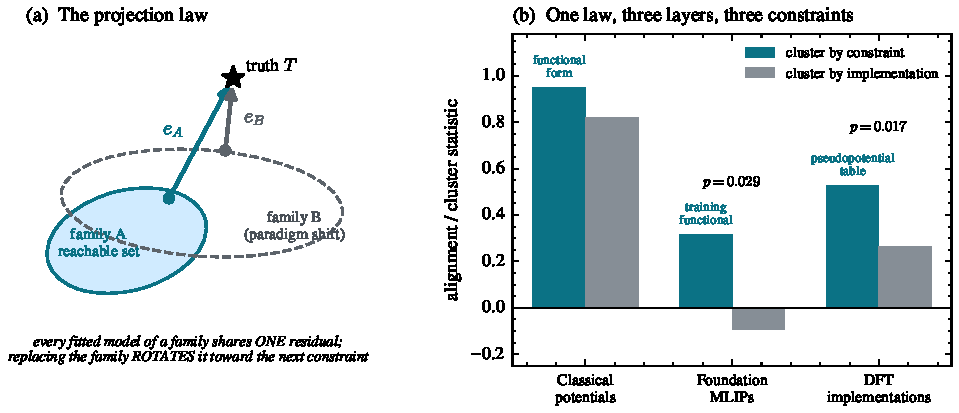
\includegraphics[width=\textwidth]{fig1_law_and_stack.pdf}
\caption{\textbf{The projection law and its three-layer test.}
(a)~A model family's reachable set fixes the residual of every well-fitted
member (Theorems~\ref{thm:cone}--\ref{thm:consensus}); replacing the family
(paradigm shift) rotates the shared residual rather than removing it.
(b)~Cluster-by-constraint versus cluster-by-implementation statistics at
three layers of one epistemic stack. Layer~1 shows within-family vs.\ pooled
reference--prediction correlation (observational); layers 2--3 show the
pre-registered cluster statistics with exact permutation $p$-values; the
registered refutation condition (implementation $>$ constraint) was not
triggered in either experiment.}
\label{fig:law}
\end{figure}

We instantiate the law at three layers of a single epistemic stack ---
classical interatomic potentials, foundation MLIPs, and the DFT
implementations that generate their training data --- because this stack
offers what few domains can: large open model ensembles, factorial structure
(the same architecture trained on two functionals; the same simulation code
run with two pseudopotential families), and references at every layer. The
empirical discovery paper for the first layer is reported separately
\citep{welcing2026instance}; here that layer serves as the observational base
of a cross-layer test.

Three methodological commitments distinguish this work, each aligned with the
verification, validation, and uncertainty-quantification practices this
journal serves. The theory core is \emph{machine-checked}: every theorem
below is verified in Lean~4 with zero unproven obligations, and a written
contract maps each theorem to the statistic that instantiates it. The two new
experiments are \emph{pre-registered}, with thresholds and explicit
refutation conditions committed to version control before any model was
executed; all threshold misses are reported as failures. And the entire
evidence chain is packaged for \emph{tiered replication}: the analysis layer
verifies from committed raw data with no machine-learning dependencies in
seconds, and the physics layer re-derives the raw data from public
checkpoints bit-exactly.

\section{Theoretical framework}
\label{sec:theory}

The mathematics of best approximation is classical
\citep{deutsch2001,kinderlehrer1980}; we claim only its epistemic application
to model ensembles and the machine-checked instantiation chain. Throughout,
$E$ is a real inner-product space (observable space), $s \subseteq E$ a model
family's reachable set, $T \in E$ the truth.

\begin{theorem}[Normal-cone criterion]\label{thm:cone}
Let $s$ be convex and $p$ a best approximation of $T$ in $s$
(i.e.\ $p \in s$ and $\|T-p\| \le \|T-q\|$ for all $q \in s$). Then the
residual $T - p$ lies in the normal cone of $s$ at $p$:
$\inn{T-p}{q-p} \le 0$ for every $q \in s$.
\end{theorem}

\begin{theorem}[Consensus]\label{thm:consensus}
Best approximations onto a convex family are unique; consequently any two
best approximations of the same target share an \emph{identical} residual.
The residual --- hence any agreement among independently fitted members ---
is determined by the (family, target) pair alone, and vanishes exactly when
the truth lies in the family.
\end{theorem}

Agreement among models sharing a constraint is therefore a measurement of the
constraint, not evidence of truth: the formal content of the qualitative
warnings of Parker \citep{parker2011} and Pirtle et al.\ \citep{pirtle2010},
and a strengthening of error-correlation dependence measures
\citep{bishop2013} in that, combined with the factorial designs of
\S\ref{sec:mlip}--\ref{sec:dft}, it identifies \emph{which} constraint binds.

\begin{theorem}[Gauge]\label{thm:gauge}
Model errors $e = b + \xi$ with shared bias $b$ and isotropic noise of scale
$\sigma$ in $d$ dimensions have error second moment with one eigenvalue
$\|b\|^2 + \sigma^2$ (bias axis) and $d{-}1$ eigenvalues $\sigma^2$, and
participation ratio
\[
\mathrm{PR}(d,\rho) \;=\; \frac{(\rho+d)^2}{(\rho+1)^2 + (d-1)},
\qquad \rho = \|b\|^2/\sigma^2 ,
\]
with $\mathrm{PR}(d,0)=d$, $1 \le \mathrm{PR} \le d$, strict decrease in
$\rho$, and the explicit collapse bound
$\mathrm{PR}-1 \le 3(d-1)/\rho$ for $\rho \ge d$.
\end{theorem}

The algebra is a one-line corollary of spiked-covariance theory
\citep{johnstone2001} and the participation ratio is a standard
effective-dimension metric \citep{gao2015}; the value here is the consilience
it enables (\S\ref{sec:classical}) and the machine-checked monotonicity that
licenses inverting measured PR into a systematic fraction
$\alpha = \rho/(\rho+1)$.

\begin{theorem}[Ribbon/consensus decoupling]\label{thm:decouple}
The participation ratio of a shared-axis ensemble $\{c_i u\}$ is $1$ for
every sign pattern of the coefficients $c_i$, while mean pairwise alignment
distinguishes them (e.g.\ $1$ vs.\ $-1/3$ for three members). PR detects the
\emph{axis}; alignment detects \emph{sign coherence}; they are distinct order
parameters.
\end{theorem}

All four theorems (and the supporting lemmas, $\sim$29 statements) are
machine-checked in Lean~4 against a pinned Mathlib, with zero \texttt{sorry}
and zero new axioms; the artifact and the theorem-to-statistic contract ship
with the replication kit (\S\ref{sec:repro}). Figure~\ref{fig:gauge}
visualizes the gauge with its classical inversion and the decoupling of the
two order parameters in live data.

\begin{figure}[t]
\centering
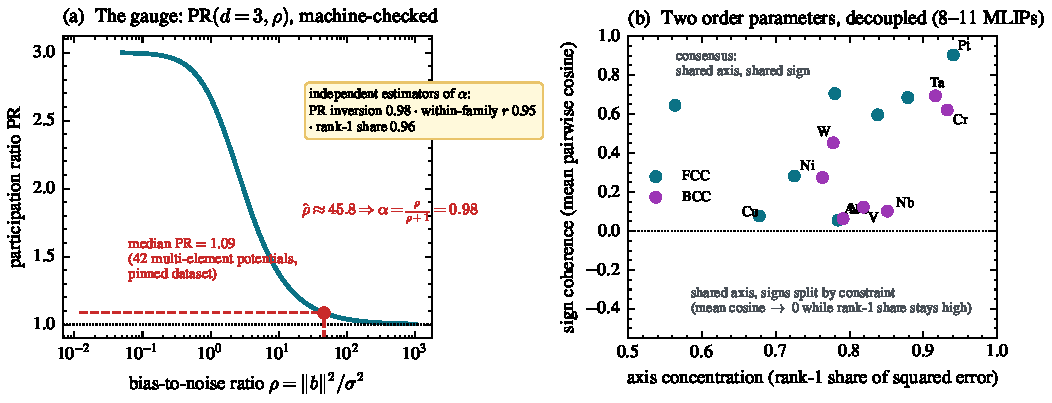
\includegraphics[width=\textwidth]{fig4_gauge_decoupling.pdf}
\caption{\textbf{The gauge and the two order parameters.}
(a)~$\mathrm{PR}(3,\rho)$ (Theorem~\ref{thm:gauge}); inverting the classical
ensemble's median $\mathrm{PR}=1.28$ gives systematic fraction
$\alpha = 0.93$, in agreement with two independent estimators
(\S\ref{sec:classical}). (b)~Per-element foundation-MLIP ensembles
($n=8$--$11$ models): axis concentration stays high for every element while
sign coherence spans the full range --- the decoupling of
Theorem~\ref{thm:decouple}. Elements whose errors split in sign by training
functional (V, Nb, W) sit low-right; consensus elements (Pt, Ta, Au) sit
top-right.}
\label{fig:gauge}
\end{figure}

\section{Layer 1: classical interatomic potentials}
\label{sec:classical}

The observational base \citep{welcing2026instance}: elastic-constant
($C_{11}, C_{12}, C_{44}$) errors of 559 classical potentials across 15 cubic
metals. Three facts matter for the law. First, error dimensionality is low
and \emph{stationary}: participation ratios of multi-element potentials
occupy $[1.0, 2.1]$ out of 3 with median $1.28$, with no trend across forty
years of potential development --- accuracy improved; geometry did not. You
cannot fit your way off a constraint surface. Second, within a
functional-form family the errors are nearly identical (within-family
reference--prediction correlation $r = 0.95$ across families vs.\ $0.82$
pooled). Third, the gauge locks: the median PR of $1.28$ inverts
(Theorem~\ref{thm:gauge}, $d{=}3$) to a systematic fraction
$\alpha \approx 0.93$, independently estimated as $0.95$ by within-family
correlation and $0.96$ by rank-one share --- three estimators, one parameter,
no tuning. The binding constraint at this layer is the functional form
itself; the oldest example is exact: central-force pair potentials satisfy
the Cauchy relation $C_{12}=C_{44}$ identically, so for any material
violating it, every pair potential's error necessarily contains the same
forced component --- the constraint dictates the direction.

We emphasize the distinction from parameter-space sloppiness: hyper-ribbon
geometry was introduced for the parameter manifolds of \emph{single} models
\citep{transtrum2011,machta2013,quinn2023,kurniawan2022}. The object here is
different --- error vectors of an ensemble of \emph{distinct} models in
observable space --- though the two pictures are related through the
projection of parameter manifolds into data space.

\section{Layer 2: foundation MLIPs --- functional vs.\ architecture}
\label{sec:mlip}

Foundation MLIPs replace the functional-form constraint with expressive
neural networks trained on DFT corpora. The law predicts the anisotropy
survives and rotates: the binding constraint becomes the training reference
theory. Qualitative inheritance of Perdew--Burke--Ernzerhof (PBE) bias ---
systematic softening shared by universal MLIPs --- has been reported
\citep{deng2025softening,yu2024}; the contributions here are the directional
quantification and the factorial attribution.

\textbf{Observation.} Three PBE-lineage models of unrelated architecture
(MACE-MP-0 \citep{batatia2024}, CHGNet \citep{deng2023}, Orb-v3
\citep{rhodes2025}) commit \emph{the same} elastic-constant errors on FCC
metals against experimental references: all-negative, $C_{44}$-dominant
(Au: $-32\%,-27\%,-79\%$), with cross-architecture cosines $0.95$--$0.99$ for
Au, Pt, Ta, Ag. An internal control excludes harness artifacts: Ni, through
the identical pipeline, has near-zero error. Across $8$--$11$ models per
element the rank-one share of squared error is $0.56$--$0.94$ --- and where
models ``disagree'' (V, Cr), they disagree by \emph{sign along the same axis}
(cosine $-0.88$), exactly the structure Theorem~\ref{thm:decouple}
distinguishes.

\begin{figure}[t]
\centering
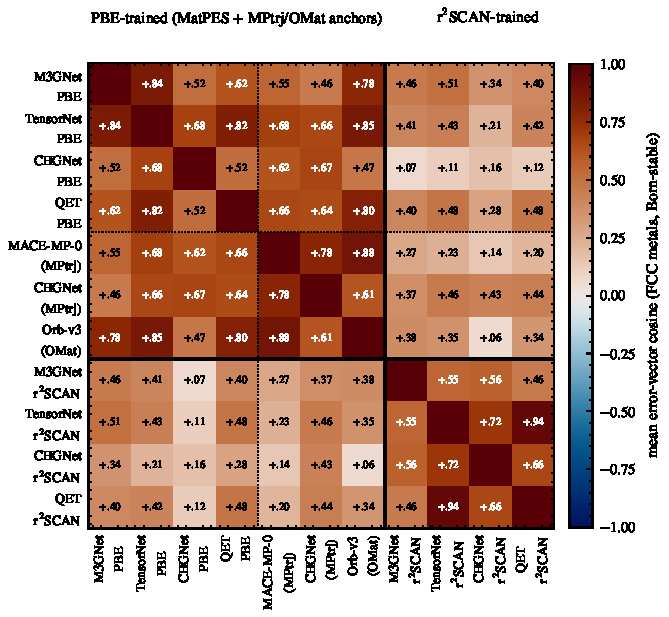
\includegraphics[width=0.72\textwidth]{fig2_mlip_matrix.pdf}
\caption{\textbf{Foundation-MLIP error geometry organizes by training
functional, not architecture.} Mean pairwise error-vector cosine over
Born-stable FCC elements for eleven models: four architectures trained on
MatPES-PBE, three PBE-lineage anchors (MPtrj/OMat training, dotted separator
= dataset axis with functional held fixed), and the same four architectures
trained on MatPES-r$^2$SCAN (solid separator). The PBE block coheres across
architectures \emph{and} datasets; the cross-functional blocks fade;
within-r$^2$SCAN pairs re-cohere (TensorNet$\times$QET $+0.94$).}
\label{fig:mlip}
\end{figure}

\textbf{Pre-registered factorial test.} The MatPES release \citep{kaplan2025}
provides one curated training distribution in two functionals (PBE,
r$^2$SCAN) with four architectures trained on each (M3GNet, TensorNet,
CHGNet, QET) --- a $4{\times}2$ crossing of constraint against
implementation. We registered thresholds and a refutation condition
(``errors cluster by architecture'') before executing any model, ran all
eight cells through one Born-screened strain-energy harness, and obtained:
clustering by functional $S_{\mathrm{func}} = +0.317$ (exact permutation
$p = 0.029$ over all 70 labelings) versus clustering by architecture
$S_{\mathrm{arch}} = -0.093$ (Fig.~\ref{fig:mlip}); the registered rotation
prediction confirmed on Au ($C_{44}$ error $-0.33 \to -0.07$) and Pt
($-0.46 \to -0.31$) under r$^2$SCAN; and the dataset-control confirmed
(MatPES-PBE models align with MPtrj/OMat-PBE anchors, median cosine $0.66$).
Two auxiliary thresholds failed as registered (within-functional median
$0.654$ vs.\ $0.70$; separation $0.085$ vs.\ $0.30$): the data revealed
\emph{nested} constraints --- Cu, Ni, Al errors reorganize by functional
(between-functional cosine down to $-0.49$, the predicted crossover), while
the $5d$ noble metals retain a shared direction across both functionals,
bound by correlation physics deeper than the PBE/r$^2$SCAN distinction. The
refutation condition was not triggered. The practical reading for transfer
learning concurs with Huang et al.\ \citep{huang2025}: GGA$\to$r$^2$SCAN
transfer is hard precisely where the two functionals' error directions
genuinely cross over.

\section{Layer 3: DFT implementations --- pseudopotential vs.\ code}
\label{sec:dft}

One layer further up, the functional itself is held fixed. The ACWF
verification effort \citep{bosoni2024,lejaeghere2016} provides
equation-of-state parameters $(V_0, B_0, B_1)$ for 384 unary crystals from
eleven pseudopotential-based methods and two all-electron codes, all PBE.
Against the all-electron average, with the FLEUR--WIEN2k split as the
per-system noise floor, the law predicts errors organize by
\emph{pseudopotential table} (the approximation actually shared), not by
\emph{simulation code} (the implementation). The dataset's factorial
structure makes the test sharp: ABINIT appears with three pseudopotential
families, Quantum ESPRESSO and CASTEP with two each, while the
PseudoDojo-0.4 table is implemented by four independent plane-wave codes.

\begin{figure}[t]
\centering
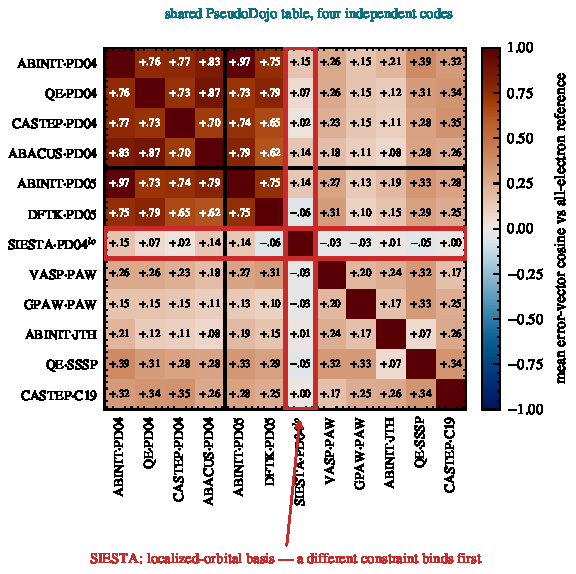
\includegraphics[width=0.78\textwidth]{fig3_acwf_matrix.pdf}
\caption{\textbf{DFT-implementation errors organize by pseudopotential table,
not simulation code.} Mean error-vector cosine in $(V_0, B_0, B_1)$ space
against the all-electron reference, over systems above the FLEUR--WIEN2k
noise floor (ACWF data, 384 unary crystals). Four independent plane-wave
codes sharing the PseudoDojo table align at $0.70$--$0.87$ (dark block); the
same code under a different pseudopotential family drops to $0.19$--$0.35$
(e.g.\ ABINIT-JTH vs.\ ABINIT-PD04). SIESTA (red frame), the one
localized-orbital-basis method, dis-aligns from its own pseudopotential
group: a different constraint binds first --- the nested-constraint
phenomenon.}
\label{fig:acwf}
\end{figure}

Pre-registered outcome: same-table--different-code alignment
$S_{\mathrm{table}} = +0.526$ versus same-code--different-family
$S_{\mathrm{code}} = +0.265$; separation $+0.261$, permutation $p = 0.017$;
refutation condition (clustering by code) not triggered
(Fig.~\ref{fig:acwf}). At pair level, four independent codes sharing
PseudoDojo-0.4 align at $0.70$--$0.87$, while ABINIT-with-JTH versus
ABINIT-with-PseudoDojo --- the same code --- drops to $0.21$. Two auxiliary
predictions failed as registered, both informatively: the within-table
consensus median ($0.459$ vs.\ $0.50$) was dragged down solely by SIESTA, the
one localized-orbital-basis code in the group, whose binding constraint is
evidently the basis set rather than the shared pseudopotential --- the
nested-constraint phenomenon again; and the registered regime prediction had
the wrong sign because between-family divergence grows on difficult elements,
which the pooled statistic conflated. A secondary observation sharpens the
law: PAW codes with \emph{different} PAW tables align at only $+0.20$ --- the
constraint is the specific frozen-core construction, not the formalism label.
Scalar reproducibility metrics \citep{lejaeghere2016,bosoni2024} cannot see
any of this structure; it lives in the directions.

\section{The conservation--rotation law}
\label{sec:law}

Table~\ref{tab:layers} assembles the stack. Three layers, three different
binding constraints, one geometric law; the two new layers tested under
pre-registration with explicit kill conditions, neither triggered. Between
layers, the direction \emph{rotates}: classical cross-family alignment has no
predictive power for MLIP alignment (Spearman $\rho = 0.26$, $p = 0.34$
across elements), because the constraint moved from functional form to
training functional; and the MLIP-layer bias direction is precisely the
reference-theory error that layer 3 isolates. Within layers, constraints
\emph{nest}: when the registered constraint is removed (r$^2$SCAN for PBE;
plane-wave pseudopotential sharing for SIESTA), residual alignment reveals
the next constraint in line (5d correlation physics; basis set). Anisotropy
is conserved throughout: at no layer, in no ensemble, under no intervention
did errors approach isotropy --- participation ratios remained far below
ambient dimension in every case, as Theorem~\ref{thm:gauge} requires of any
family whose systematic error dominates its fitting scatter.

\begin{table}[t]
\centering
\caption{The projection law across one epistemic stack. Each row: an ensemble
of models, the constraint the law identifies as binding, the clustering
evidence (constraint vs.\ implementation), and the registered refutation
condition's status.}
\label{tab:layers}
\small
\begin{tabular}{@{}lllll@{}}
\toprule
Layer & Ensemble & Binding constraint & Evidence & Kill condition \\
\midrule
Classical IPs & 559 potentials & functional form & within-family $r{=}0.95$; PR invariant 40 yr & (observational) \\
Foundation MLIPs & $4{\times}2$ MatPES $+$ anchors & training functional & $S_{\mathrm{func}}{=}{+}0.317$ vs ${-}0.093$, $p{=}0.029$ & not triggered \\
DFT codes & 12 ACWF methods & pseudopotential table & $S_{\mathrm{table}}{=}{+}0.526$ vs ${+}0.265$, $p{=}0.017$ & not triggered \\
\bottomrule
\end{tabular}
\end{table}

The closest antecedents are the persistence of shared biases across climate
model generations \citep{tian2020,knutti2013}, the convergence of training
trajectories onto shared low-dimensional manifolds \citep{mao2024}, and
representation convergence across architectures \citep{huh2024}; none states
conservation-plus-rotation as a law, and none possesses the factorial
constraint-vs-implementation evidence presented here.

\section{Related work}
\label{sec:related}

\textbf{Ensemble dependence across fields.} The climate community has the
deepest tradition here. Pirtle et al.\ \citep{pirtle2010} and Parker
\citep{parker2011} argued qualitatively that multi-model agreement may
reflect shared construction; Bishop and Abramowitz \citep{bishop2013} made
dependence operational through pairwise error correlation under the
replicate-Earth paradigm, with the elegant null that truly independent models
would correlate at $0.5$ through the shared observations;
\citep{abramowitz2019} review the resulting weighting and sub-selection
machinery, \citep{knutti2017} implement performance-plus-independence
weighting, \citep{boe2018} traces similarity to literal component replication
across modeling centers, and \citep{sanderson2015,brands2022} place
inter-model error in low-dimensional EOF coordinates. Our normal-cone theorem
supplies the mechanism beneath these practices --- dependence is not merely
shared code but shared \emph{reachable set} --- and the factorial designs add
what error correlation alone cannot: identification of \emph{which} shared
element binds. The persistence of the double-ITCZ bias across three CMIP
generations \citep{tian2020} reads, in our terms, as a conservation
observation awaiting its rotation experiment.

\textbf{Machine learning.} That independently trained networks agree beyond
chance is quantified by error consistency \citep{geirhos2020} and model
similarity \citep{mania2019}; ensemble members cluster in prediction space
\citep{fort2019} despite weight-space diversity, which is why deep-ensemble
uncertainty \citep{lakshminarayanan2017} inherits the shared component as
unaccounted bias --- the ambiguity decomposition of Krogh and Vedelsby
\citep{krogh1995} already showed ensemble spread bounds only the variance
term. Disagreement tracks the training procedure's shared bias
\citep{jiang2021}, and accuracy- and agreement-on-the-line
\citep{miller2021,baek2022} exhibit one-dimensional collective structure
under distribution shift. Most complementary is underspecification
\citep{damour2022}: it studies how equally-fitted models \emph{differ} along
directions the family and data leave unconstrained --- our noise term $\xi$
--- whereas the projection law studies what they \emph{share} --- the bias
$b$. Theorem~\ref{thm:decouple} is precisely the statement that these are
separate order parameters, measurable separately. Representation convergence
across architectures \citep{huh2024} and shared training manifolds
\citep{mao2024} are the trajectory- and representation-space cousins of our
observable-space result.

\textbf{Materials simulation.} Frederiksen et al.\ \citep{frederiksen2004}
pioneered ensembles of interatomic potentials for error estimation --- spread
as uncertainty; the law identifies exactly the component spread misses (the
shared residual) and supplies the diagnostic for when it dominates
(alignment). Shared softening of universal MLIPs is documented
\citep{deng2025softening,yu2024}, and Huang et al.\ \citep{huang2025} report
that GGA$\to$r$^2$SCAN transfer is hampered by poor inter-functional
correlation --- our factorial result gives that observation a geometric form.
DFT reproducibility is measured by scalar and curve metrics
\citep{lejaeghere2016,bosoni2024}; the directional structure of
\S\ref{sec:dft} is invisible to those metrics by construction.
Parameter-space sloppiness of single models
\citep{transtrum2011,machta2013,quinn2023,kurniawan2022} is the intellectual
ancestor of this work; we re-emphasize that the object here --- error vectors
of an ensemble of distinct models in observable space --- is different from,
though related to, the parameter manifold of any one of them. The
participation ratio is a standard effective dimension \citep{gao2015} and the
gauge algebra is spiked-covariance theory \citep{johnstone2001}; the
best-approximation mathematics is classical
\citep{deutsch2001,kinderlehrer1980}.

\textbf{What is new here} is the combination: the error-vector geometry of
model ensembles as the measured object; factorial
constraint-vs-implementation designs with pre-registered refutation
conditions at two layers of one stack; the conservation--rotation law; and a
machine-checked theory chain bound to the measurements by a written contract.

\section{Discussion: implications for benchmarking, VVUQ, and calibration}
\label{sec:implications}

\textbf{Calibration without retraining.} Because the shared error is one
direction, one correction vector per (element, observable) repairs every
model in the family at once: a rank-one correction removes ${\sim}96\%$
(median) of foundation-MLIP elastic error. The correction is family-level:
it transfers to models not yet trained, so long as they share the
constraint.

\textbf{A trust rule for ensemble UQ.} Cross-model alignment is a zero-cost
diagnostic: high alignment $\Rightarrow$ the ensemble is constraint-bound,
calibratable, and its spread \emph{understates} uncertainty; low alignment at
the noise floor $\Rightarrow$ genuine convergence (the Ni control); low
alignment far above the floor $\Rightarrow$ the constraint is heterogeneous
(magnetic BCC metals; difficult elements across pseudopotential tables) and
no shared correction exists.

\textbf{Benchmark design.} Leaderboards that pool across families average
away the very direction that identifies what to fix. Reporting error
\emph{directions} stratified by candidate constraints --- the factorial
pattern used here --- converts benchmarking from scoring into diagnosis.
This is directly actionable for materials data infrastructure: benchmark
records should carry the error vector, not only its norm.

\textbf{Reading consensus.} Where ground truth is delayed (materials
discovery campaigns, extrapolative simulation), inter-model agreement should
be priced as a measurement of shared constraint; the factorial designs show
how to estimate \emph{which} constraint, today, from models alone.

\section{Limitations}
\label{sec:limits}

The formal chain covers convex reachable sets and deterministic
bias-plus-noise spectra; smooth non-convex families (local normal cones) and
the finite-sample step from noisy ensembles to the exact second moment are
standard but unformalized. The MLIP layer uses one validated harness, fifteen
cubic elemental metals, and elastic observables; the DFT layer inherits
ACWF's protocol choices. Four of nine registered auxiliary thresholds across
the two experiments failed and are reported as failures; in each case
post-hoc analysis attributes the miss to nested constraints, and those
attributions are hypotheses for the next registration round, not confirmed
claims. The law itself makes its next predictions cheap to test: an
r$^2$SCAN-trained model from a fourth architecture must join the r$^2$SCAN
cluster; a plane-wave implementation of any new pseudopotential table must
align with its table, not its code; and axis-based statistics (mandated by
Theorem~\ref{thm:decouple}) should replace signed-cosine thresholds.

\section{Reproducibility}
\label{sec:repro}

Both experiments were pre-registered with thresholds and refutation
conditions committed to version control before execution (commits
\texttt{dffbe595} and \texttt{ebf39e33}); all analysis is replayable from a
two-tier kit in which Tier~1 verifies every statistic in this paper from
committed raw data using only NumPy/SciPy in seconds, and Tier~2 re-derives
the raw elastic constants from public checkpoints through a frozen harness
(bit-exact on revalidation). The Lean~4 artifact (four theory files,
$\sim$29 machine-checked statements, zero \texttt{sorry}, zero new axioms,
pinned Mathlib) and the theorem-to-statistic contract accompany the kit. The
harness was validated by independent energy- vs.\ stress-method agreement
($\le 2.4\%$), bit-exact regression, and strain-window stability. ACWF data
are from the public archive of \citep{bosoni2024}; MatPES checkpoints from
\citep{kaplan2025}.

\section*{Declarations}

\textbf{Funding.} This work was supported by Lupine Science.

\textbf{Competing interests.} The author declares no competing interests.

\textbf{Data and code availability.} The two-tier replication kit (raw data,
analysis scripts, frozen harness), the pre-registration documents with their
commit hashes, the Lean~4 formal artifact, and figure-generation scripts are
available in the project repository and will be archived with a DOI at
acceptance. Third-party data: ACWF verification archive \citep{bosoni2024};
MatPES checkpoints \citep{kaplan2025}; OpenKIM/NIST classical-potential data
as described in \citep{welcing2026instance}.

\textbf{Author contributions.} A.W.\ conceived the study, performed the
research, and wrote the manuscript.

\textbf{Use of AI assistance.} AI assistance (Anthropic Claude) was used
under the author's direction for statistical verification and recomputation,
Lean proof engineering, literature triage, figure generation, and drafting;
all scientific claims and decisions were reviewed and approved by the author,
who takes sole responsibility for the content.

\bibliographystyle{unsrtnat}
\bibliography{references}

\end{document}
